\documentclass[a4paper,UTF8]{article}
\usepackage{ctex}
\usepackage[margin=1.25in]{geometry}


\usepackage{url}
\usepackage{enumerate}

\usepackage{algorithm}
\usepackage{algorithmic}
\renewcommand{\algorithmicrequire}{\textbf{Input:}}
\renewcommand{\algorithmicensure}{\textbf{Output:}}


\begin{document}
\title{综述. 特征选择方法}
\author{MF1733062 万晨 \url{weanl_jc@163.com}}
\maketitle

\section*{1. 介绍}
  FS在ML中能解决那些问题?已经解决得怎么样了?还有那些问题?feature construction = FS + FE
  特征选择(Feature, Variable and Attribution Selection),是机器学习中feature construction的重要组成部分。
  在筛选原始数据,构造有用的特征集合方面,特征选择不同于特征提取(Feature Extraction):后者会通过线性或非线性的方式
  从原始数据中构造出全新的特征,具有特征学习和表示学习的能力
  ["Representation Learning: A Review and New Perspectives"];
  特征选择通过设计一些简单高效或者精致巧妙的方法,实现从原始特征集合中选出最优的特征子集,能够保持特征对应的原始物理意义。
  所谓最优特征子集,理论上定义为没有信息丢失的最小特征子集,以Markov blanket的形式给出
  [D. Koller, Toward optimal feature selection]
  [C.Aliferis, Local causal and markov blanket induction for causal discovery and feature selection];
  实际中理论的ground-truth很难找,所以经验上一般我们用预测器性能(如分类器的精度)来评估特征子集的选择结果。
  特征选择一直以来是一个重要的课题:为了分析特征间相关性,早期[Blum and langley,1997,Kohavi and John,1997]等
  在1997年提出了特征选择方面课题研究,当时大多数应用领域下特征维数还不超过40。后续基因序列分析和web文本分类等典型应用
  不断推动特征选择课题研究:[2001, Feature selection for high-dimensional genomic microarray data]
  针对高维的染色体序列数据提出了给予特征选择的基因分析方法,
  [2015, Deep Feature Selection: Theory and Application to Identify Enhancer and Promoters]将深层神经网络
  应用到特征选择中,实现了基因Enhancer和Promoter的有效分析。目前特征选择研究有两大趋势:
  第一,应对各种结构化和非结构化的数据设计出一套较为通用的方法,决策树类和深层神经网络类在特征选择方面的改进是不错的解决方法,
  [Feature Selection via Regularized Trees]就是通过修改单棵树的构造算法实现基于随机森林的Ensemble类的特征选择方法;
  第二,应对curse of dimensionality,设计复杂度较低的算法,有效地处理高维数据,改进现有的算法以及组合使用一些简单的算法
  都是很好的思路。

  在数据处理中,应用特征选择方法概括起来有如下优势:
  \begin{itemize}
    \item 可以过滤无关特征:
    采集过程可能引入数据噪声,从而影响后续的数据处理;同样与任务显著的无关特征(irrelevant)也可以认为是噪声,
    特征选择方法一定程度上可以过滤这一部分噪声;

    \item 可以剔除冗余特征:
    相当部分特征虽然与任务相关,但互相之间存在显著的冗余关系(redundant),特征选择方法可以依据实际需求选出代表性的特征,
    降低冗余;

    \item 可以实现特征重要性的评估:
    一些带有指标(如相关系数、权值)或其他“得分”的特征选择方法,可以在选出的特征子集中按指标或“得分”对特征进行重要性排序。

  \end{itemize}

  文章接下来的章节安排:section 2总结三类方法:过滤式(filter)、包裹式(wrapper)和嵌入式(embbedding),以及经典算法;
  section 3介绍最近流行的深度学习在特征选择方面的应用以及特征选择针对时序分析方面的方法;
  section 4介绍我们尝试设计的方法以及在数据集上的评价。

  过滤式:(线性相关系数、互信息系数、relief and relief-F、combination)

  包裹式:(一般子集搜索策略)





\section*{2. 过滤式、包裹式与嵌入式}
  特征选择的形式化定义:
  首先将样本空间定义为一个$ N $维的随机变量$ X = (X_{0}, X_{1}, ... , X_{N-1})$,
  其服从一定的概率分布,通常认为样本实例(数据)都是该概率分布采样所得;
  特征全集$ S = \{X_{0}, X_{1}, ... , X_{N-1}\} $,特征选择考虑的是如何有效地除去无关和冗余的特征,
  筛选得到”最优”特征子集$ S^{*} \subset S $[?]。
  显然,暴力地遍历$ S $所有子集会遇到组合爆炸,是不可行的。实际设计中,常采用如下思路进行搜索:

  \begin{itemize}

    \item 产生初始候选特征子集,进行下一步;
    \item 评价候选特征子集,如果达到终止条件终止搜索,否则进行下一步;
    \item 基于上一步评价结果,生成新候选特征子集,返回上一步。

  \end{itemize}
  由上,特征选择方法可以依据新候选特征子集的方法(Search Strategies)进行分类,通常有Complete、Sequential
  和Random等策略,但这种分类方法不是主流的划分方法。主流的分类方法是依据候选子集的评价方法(Evaluation Criteria)
  对特征选择方法进行分类,简单地说,用独立于学习器的方法进行评价的称为过滤式方法,用学习器的性能进行评价的称为包裹式方法,
  本章节先介绍这两种很早被提出的方法。接着我们还会介绍后续巧妙独特的嵌入式方法,不同于前两种前两类方法,
  嵌入式方法将特征选择嵌入到学习器的训练过程中。


\subsection*{2.1 过滤式方法}
  算法的统一形式(见Algorithm 1),  算法中$ eval(S_{0}, D, M)$说明过滤式采用独立的评价方法,下面介绍几种常见的方法。

  \begin{algorithm}
    \caption{过滤式算法}
    \begin{algorithmic}[1]
      \REQUIRE 数据集空间$D(F_{0}, F_{1},..., F_{N-1})$;初始特征子集$S_{0}$;停止条件标准$\delta$;
      \ENSURE 优化子集结果$S_{best}$

      \STATE $S_{best}=S_{0}$
      \STATE $\gamma_{best}=eval(S_{0},D,M)$          $//$ M是独立的评价方法

      \WHILE{($\delta$ is not reached)}
        \STATE $S=generate(D)$
        \STATE $\gamma=eval(S,D,M)$
          \IF{($\gamma$ is better than $\gamma_{best}$)}
            \STATE $\gamma_{best}=\gamma$
            \STATE $S_{best}=S$
          \ENDIF
      \ENDWHILE

      \RETURN{$S_{best}$}

    \end{algorithmic}
  \end{algorithm}


\subsubsection*{2.1.1 基于pair-wise的度量}
  线性相关系数、信息熵方法及MIC、relief-F

  在统计学中,常用线性相关系数(Pearson correlation coefficient)衡量两个随机变量间线性相关性。
  若定义两个随机变量$ A, B $,则可有$M$个采样$ A: a_{0},...,a_{M-1}; B: b_{0},...,b_{M-1}$
  计算出两随机变量间的线性相关系数(的估计值):
  $$  r_{AB} = \frac{\sum_{i=0}^{M-1}(a_{i}-\overline{a})(b_{i}-\overline{b})}
  {\sqrt{\sum_{i=0}^{M-1}(a_{i}-\overline{a})^2}\sqrt{\sum_{i=0}^{M-1}(b_{i}-\overline{b})^2}}$$

  $ r_{AB} $在$ [-1,1]$上取值,一般做如下判断:如果$ \mid{r_{AB}}\mid<0.2$,认为A和B显著地没有线性相关性;
  如果$ \mid{r_{AB}}\mid>0.8$,认为A和B显著地有线性相关性。
  在特征选择中一般做如下应用:令$ A=X_{i},i=0,1,...,N-1, B=Y$,其中$Y$为监督学习下给出的数据标签对应的随机变量
  称为标签变量,满足现实的映射关系$Y=f(X)$;然后计算$ r_{AB} $,即计算$N$个特征和标签变量的线性相关系数,
  从而剔除一些$\mid{r_{AB}}\mid$过小的特征。该方法在线性假设下能过滤一些无关特征,计算简单应用广泛。
  这里需要注意的是该方法由如下应用前提:$A,B$为连续的随机变量;$A,B$应通过正太分布检验,即大致呈正太分布。

  线性相关系数给我们提供了这样一条思路:逐个考虑特征和标签变量间的关系并进行筛选特征,实际上每次计算的是两个随机变量间的关系,
  该类方法是pair-wise的,定义良好的度量关系是关键。
  在信息论中,基于信息熵的信息增益是常用的衡量两个随机变量可以互相预测(predict)性,对于随机变量$ A, B $,
  采用归一化的衡量指标symmetrical uncertainty[?]:
  $$ SU(A, B) = 2 \frac{IG(A \mid B)}{H(A)+H(B)} $$
  其中$IG(A \mid B)=H(A)-H(A \mid B)$为信息增益,对于$A,B$是对称的;
  $H(A)=-\sum_{i}P(a_{i})log_{2}(P(a_{i}))$为$A$的信息熵,$H(B)$计算类似;
  $H(A \mid B)=-\sum_{j}P(b_{j})\sum_{i}P(a_{i} \mid b_{j})log_{2}(P(a_{i} \mid b_{j}))$为观测到$B$的条件下
  $A$的信息熵,可以证明对于$A,B$是对称的。
  这种归一化的信息增益方法,克服了线性相关系数的较为苛刻的前提假设:不需进行正太分布检验,能很好地度量变量间的非线性关系,
  同时对于连续的变量可以进行离散化处理以便于计算。当然该方法通用性增加的同时,计算量明显调高了不少。

  机器学习中,应对分类任务常用Relief(Relevant Feature)进行过滤式的特征选择[Kira and Rendell, 1992]。
  延续上述思路,Relief本质上也是一种度量关系,基于样本的分类标签,可以计算出第$j$个特征的度量得分:
  $$ \delta^{j}=\sum_{i}-diff(x_{i}^{j},x_{i,nh}^{j})^{2}+diff(x_{i}^{j},x_{i,nm}^{j})^{2} $$
  Relief和多分类扩展的Relief-F方法,都是考察最近同类样本$x_{i,nh}$和最近异类样本$x_{i,nm}$,依据类似上面的式子
  计算第$j$个属性对样本分类的性能,以此作为该特征的度量指标。

  上述方法可以总结为基于pair-wise的度量,显然忽略了特征的组合影响,所以通常用来独立地过滤那些显著无关的特征,
  不能解决特征冗余的问题;另外这类方法天然的有度量指标,在实际中可以评估特征重要性。


\subsubsection*{2.1.2 组合方法}

[2003, Feature Selection for High-Dimensional Data: A Fast Correlation-Based Filter Solution]
对于分类任务的特征选择提出了基于纯过滤式方法的FCBC Algorithm,经过精心的设计可以很好地解决特征冗余的问题。
算法采用的是(2.1.1)中归一化的信息增益$SU(A,B)$作为相关关系度量,对应记作$SU_{A,B}$;
定义了主导特征(Predominant Feature)。
记特征全集$S$,候选特征子集$S^{*}$,在考虑把特征$F_{i}$加入$S^{*}$时,$F_{i}$必须为主导特征;
所谓主导特征,首先满足$SU_{i,C} > \delta$,如果还满足在$S^{*}$中不存在$F_{j}$
使得$SU_{j,i}>SU_{i,C}$,那么$F_{i}$是主导特征,
如果不满足第二个条件可以用存在的特征$F_{j}$构建redundant peer集合$S_{P_{i}}$,
然后依据算法缩减该集合,如果能缩减为空集,$F_{i}$也是主导特征。具体算法见[?]。

如果样本的数量规模为$N$,特征规模为$M$,FCBC算法的时间复杂度为$O(MNlogN)$,是比较快速的特征选择算法,
能很好的应用到大量的高维数据。文章用有上千维特征数据的分类任务作为算法的评估,经验说明该精心设计的算法能取得不错的精度。






\subsection*{2.2 包裹式方法}
算法的统一形式(见Algorithm 1):

\begin{algorithm}
  \caption{包裹式算法}
  \begin{algorithmic}[1]
    \REQUIRE 数据集空间$D(F_{0}, F_{1},..., F_{N-1})$;初始特征子集$S_{0}$;停止条件标准$\delta$;
    \ENSURE 优化子集结果$S_{best}$

    \STATE $S_{best}=S_{0}$
    \STATE $\gamma_{best}=eval(S_{0},D,A)$          $//$ A是基于学习器性能的评价方法

    \WHILE{($\delta$ is not reached)}
      \STATE $S=generate(D)$
      \STATE $\gamma=eval(S,D,A)$
        \IF{($\gamma$ is better than $\gamma_{best}$)}
          \STATE $\gamma_{best}=\gamma$
          \STATE $S_{best}=S$
        \ENDIF
    \ENDWHILE

    \RETURN{$S_{best}$}

  \end{algorithmic}
\end{algorithm}


包裹式方法用学习器的性能对候选特征子集进行评价,好处在于可以方便地对候选子集所有特征一起做评价,
也就是生成新的候选子集都要训练一遍学习器。
%包裹式方法在解决特征冗余方面很有优势,但
显然多次训练学习器的计算开销是巨大的,所以通常包裹式方法关注的是优化子集搜索(新候选子集生成)策略,
提高搜索效率。

(感觉wrapper要凉了)较为简单地说一些方法。


\subsection*{2.3 嵌入式}

嵌入式方法是继过滤式和包裹式后提出的特征选择方法,将特征选择嵌入到学习器的训练过程,通常该类算法计算复杂度比包裹式方法低,
同时能获得不错的特征子集。
要插入吗[????]
嵌入式方法结合了前两种方法的优势,是十分流行的方法,前人基于已有的学习器模型提出了一些精致的方法。

\subsubsection*{2.3.1 基于常用模型}

lasso类(elastic net regularization)、SVM-RFE(Recursive Feature Elimination)、Regularized decision tree

首先基于回归任务中基本的学习器模型——线性回归(linear regression),[Tibshirani, 1996]
提出了Lasso(least absolute shrinkage and selection operator)。
Lasso通过在线性回归损失函数中添加$l_{1}-norm$正则化项,
降低模型过拟合风险($l_{2}-norm$的岭回归就是被提出来降低过拟合风险)的同时得到的稀疏权值向量可以作为特征选择的依据。
下面给出Lasso的形式化定义:
$$ min \sum_{i}(y_{i}-\textbf{w}^{T}\textbf{x}_{i})+\lambda \parallel \textbf{w} \parallel _{1} $$
参数$\lambda>0$,该值越大对$\textbf{w}$的稀疏性约束越强,可以通过交叉验证的方式选取适当的值;
算法收敛下得到的权值向量$\textbf{w}$一般是稀疏的,即$\textbf{w}$的各个分量$w_{i}$大部分为接近零的值,
而$w_{i}$对应的意义是特征$X_{i}$在线性模型中的权重,自然地零值或接近零值对应的特征可以被舍弃,
这样在线性模型训练完成的同时也完成了特征选择过程。
实际上,上述给出的是basic lasso方法,后续在实践中遇到一些应用问题,做了一些改进和推广。
记样本数量为$M$,特征维度为$N$,当应用场景中$N>M$或$N>>M$时,basic lasso选出的特征数量不会超过$M$,
这容易导致有用特征信息的丢失;
[2005,Zou and Hastie]提出elastic net的正则化,同时使用了$l_{1}-norm$和$l_{12}-norm$进行正则化:
$$ min \sum_{i}(y_{i}-\textbf{w}^{T}\textbf{x}_{i})+
\lambda_{1} \parallel \textbf{w} \parallel _{1} +\lambda_{2} \parallel \textbf{w} \parallel _{2} $$
实际上基于elastic net正则化的lasso在$l_{1}-norm$约束的稀疏性和$l_{2}-norm$约束
对特征间强相关问题的处理取得了不错的平衡。

另外应对诸如基因序列分析这类问题,背景约束一组特征必须被选进最优特征子集。
[2006,Yuan and Lin]提出了Group lasso,把约束的特征组对应的权值作为新的正则化项
[Model Selection and Estimation in Regression with Grouped Variables]。
该方法满足特征组约束条件同时能很好的考虑多个特征对任务的组合影响,在组合影响成为主导因素的场景中有很好的应用。


对于分类任务,我们介绍基于十分流行的支持向量机(SVM)模型的嵌入式特征选择方法——SVM-RFE(Recursive Feature Elimination)。
首先给出经典的支持向量机的公式定义:
$$ min \frac{1}{2}\parallel \textbf{w} \parallel^{2} $$
$$ s.t. y_{i}(\textbf{w}^{T}\textbf{x}_{i}+b)>=1 $$
SVM-RFE是循环删除特征的过程,每一轮用当前未被删除的特征训练学习器SVM,并得到特征$X_{i}$的权值$w_{i}$,
然后每个特征按照得分$C_{i}=w_{i}^{2}$进行排序,在该轮训练中删除得分最小的特征。
用该算法进行特征选择时,可以制定最后保留的特征子集的大小。SVM-RFE最早提出来被应用到医学癌症分析领域,取得了不错的
分析效果,究其原因是SVM良好的分类性能,也从侧面说明了嵌入式特征选择的性能很大程度上依赖于学习器模型。
[Guyon, Gene Selection for Cancer Classification using Support Vector Machines]


延续上述思路,我们介绍基于决策树或判定树(Decision Tree)的嵌入式特征选择方法——Regularized Trees。
该方法的思想是在单棵决策树的构造过程中加入正则化项,目的是尽量减少划分中设计的特征的种类数;
因为划分中用到的特征可以认为是重要的特征,那么在划分过程中尽量使用之前的划分过程中用到的特征,
那么最后决策树构造完成时划分用到的所有特征种类数是相对少的。
Regularized Trees的做法是惩罚性地对于当前划分中可能用到的全新的特征种类计算得到的信息增益乘上一个小于1的系数,
下面是具体算法:

\begin{algorithm}
  \caption{正则化决策树算法,递归调用$S=tree(data,S,\lambda)$}
  \begin{algorithmic}[1]

    \STATE $gain^{*}=0$
    \STATE $count=0$

    \FOR{$m=1:M$}
      \STATE $gain_{R}(X_{m})=0$
      \IF{$X_{m} \in F$}
        \STATE $gain_{R}(X_{m})=gain(X_{m})$
      \ENDIF

      \IF{$X_{m} \notin F$ and $count<\lceil \sqrt{M} \rceil$}
        \STATE $gain_{R}(X_{m})=\lambda \cdot gain(X_{m})$ $//$ 正则化惩罚
        \STATE $count=count+1$
      \ENDIF

      \IF{$gain_{R}(X_{m})>gain^{*}$}
        \STATE $gain^{*}=gain_{R}(X_{m})$
        \STATE $X^{*}=X_{m}$
      \ENDIF

    \ENDFOR

    \IF{$gain^{*}=0$}
      \STATE make this node as a leaf and return $S$
    \ENDIF

    \IF{$X^{*} \notin F$}
      \STATE $F=\{F,X^{*}\}$
    \ENDIF
    \STATE split $data$ into $\gamma$ child nodes by $X^{*}$:$data_{1},...,data_{\gamma}$

    \FOR{$g=1:\gamma$}
      \STATE $S=tree(data_{g},S,\lambda)$
    \ENDFOR

    \RETURN $S$
  \end{algorithmic}

\end{algorithm}


Regularized Trees在全体数据集中随机采样部分数据构造单棵决策树,类似于esemble的方法:
\begin{algorithm}
  \caption{集成化算法,$S=ensemble(data,S,\lambda,nTree)$}
  \begin{algorithmic}[1]

    \FOR{$iTree=1:nTree$}
      \STATE select $data_{i}$ from $data$ with some criteria
      \STATE $S=ensemble(data,S,\lambda)$
    \ENDFOR
  \end{algorithmic}


\end{algorithm}

决策树对连续值一般做离散化处理。得益于决策树模型的优势,Regularized Trees是个不错的特征选择方法,
劣势是计算量比SVM和Lasso类的方法大很多。[Feature Selection via Regularized Trees]


\section*{3 深度模型}


\subsection*{3.1 理论模型分析}

本文以上介绍了不同需求下的一些特征选择方法,可以说特征选择领域的方法繁多,虽说以候选特征子集的评价标准分为了三大类,
但面对一些具体问题,有时候我们还是很难选择合适的方法。下面我们提出关于特征选择理论模型分析,给实际应用给出理论依据。

section 1中说明的特征选择要尽量保证不会丢失信息,即理论上保留信息的完整性。[combining multiple feature Selection
methods and deep learning for high-dimensional data]中贡献性地提出了基于学习器学习的目标模型类型选择
合适的特征选择方法。所谓目标模型就是实际任务,可以表示为特征空间到标签值空间的映射函数:
$$y_{i}=f(x_{i})=\beta_{0}+\beta x_{i}+\sum_{j}{\alpha_{j} g_{j}(x_{i}^{1},...,x_{i}^{p})}
+\sum_{k}{\gamma_{k} h_{k}((x_{i}^{1},...,x_{i}^{p}))}+\varepsilon_{i}$$
其中$x_{i}$是来自数据集空间$D(F_{0}, F_{1},..., F_{N-1})$的样本,$y_{i}$是真实标签值;$\beta_{0}$为常数,
$\beta x_{i}$和$h_{k}((x_{i}^{1},...,x_{i}^{p})$描述的都是线性关系,前者侧重的是单个特征的相关性,
后者侧重的是多个特征线性叠加对$y_{i}$的影响,如$h(x_{i}^{1},x_{i}^{2})=x_{i}^{1}x_{i}^{2}$;
$g_{j}(x_{i}^{1},...,x_{i}^{p})$描述的是多个特征非线性叠加对$y_{i}$的影响,
如$g(x_{i}^{1},x_{i}^{2})=x_{i}^{1}sin(x_{i}^{2})$.

所以依据上式,对不同实际的学习任务,我们可以因地制宜地选择合适的特征选择方法:线性项为主导影响时可以采用如Lasso这样的
基于线性模型的方法;组合复杂项为主导影响时可以采用集成化的正则决策树;当然简单的单个线性或非线性特征为主要影响时完全可以
用过滤式中pair-wise的方法。


\subsection*{3.2 深度学习方法}
深度学习本质上是神经网络的新一轮复兴,无论在学术界还是在工业界都很受欢迎。将deep learning应用到特征工程称为feature
learning,其中包括了从原始数据到学习器利用的数据之间的数据预处理、特征提取和特征选择。其实feature learning研究的
动机是基于这样一条定律从现实世界构造的抽象数据决定了学习器的性能上界,所以构造特征是一项十分重要的工程(广义上说,机器
学习中metric learning和kernal learning也是这方面的努力)。现实中从高维数据中构造有用的特征集,为了克服盲目性
需要大量的领域知识,而且通常这项工作是复杂且昂贵的。一个典型的例子是图片识别,经验地构造特征甚至是不可行的(PCA等分析
方法可以解决问题)。层结构经过精心设计的深度网络可以自动的完成很多特征工程方面的任务,这也是feature representation
的研究热点。不过由于网络自身结构,不会严格的保留变换前后特征的一一对应关系,所以目前feature learning方面绝大部分
属于特征提取,如图像的卷积层提取、AutoEncoder和Sparse Coding等。

[Deep Feature Selection:]用深层的神经网络做特征选择,设计的网络结构如下:

\begin{figure}[!htbp]
  \centering
  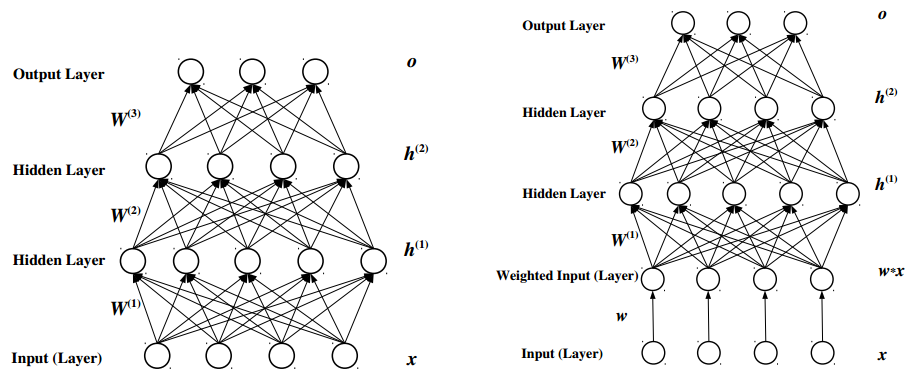
\includegraphics[scale=0.4]{DFS.png}
  \caption{深度特征选择}
\end{figure}
图中左边为常用的深层网络DNN,在输入层直接将数据输入;右边是文章设计的网络结构:在数据输入层和第一个隐层间加了一层
带权值的输入层Weighted Input Layer,其中$w=(w_{0},...,w_{N-1})$的每个元素描述样本对应特征的对标签输出的
影响重要性,网络训练完成后$w$的零范数同来做特征选择,即只选取非零$w_{i}$对应的特征。

该方法可以总结为DFS=DNN+FS,为了获得稀疏的$w=(w_{0},...,w_{N-1})$文章也构造了输出层带有正则化的损失函数,具体
参考文献,另外作者也公开了在Theano上实现的代码供参考。\cite{wiki}


\subsection*{3.3 时序数据处理方法}

未完待续。。。



\section*{4 方法与评估}

\subsection*{4.1 问题定义与数据集}

\subsection*{4.2 思路和方法}

\subsection*{4.3 初步结果}



\section*{5 工作总结}














\bibliographystyle{plain}
\bibliography{report}








\end{document}
